La inteligencia artificial es la mejor solución para resolver el problema de la ambigüedad. Al entrenar e implementar una red neuronal, podemos lograr precisiones casi similares a la de los seres humanos, como lo detallamos en la sección anterior.

\subsection{Implementación Simple de AI}

El objetivo de esta experimentación es poder transmitir un poco de lo que se puede hacer con esta tecnología. En este caso, implementaremos una pequeña red neuronal para identificar si una titular de una noticia contiene 'sarcasmo' o no. Para luego, finalizar el proyecto con algunos futuros cambios que se podrían hacer para adaptarlo a gramáticas.

La siguiente implementación fue creada por Rishabh Misra \cite{NLPinTensorFlow}.

\begin{lstlisting}[style= mystyle, language=Python]
import json
import tensorflow as tf

from tensorflow.keras.preprocessing.text import Tokenizer
from tensorflow.keras.preprocessing.sequence import pad_sequences
\end{lstlisting}

En este caso utilizaremos la librerías de TensorFlow para hacer esto posible.

\begin{lstlisting}[style= mystyle, language=Python]
vocab_size = 10000
embedding_dim = 16
max_length = 100
trunc_type='post'
padding_type='post'
oov_tok = "<OOV>"
training_size = 20000
\end{lstlisting}

En primer lugar, tenemos que definir ciertos parámetros como el tamaño del vocabulario, la longitud máxima de una oración y el tamaño de nuestro entrenamiento.

\begin{lstlisting}[style= mystyle, language=Python]
!wget --no-check-certificate \
    https://storage.googleapis.com/laurencemoroney-blog.appspot.com/sarcasm.json \
    -O /tmp/sarcasm.json
\end{lstlisting}

Para ese experimento, utilizaremos un archivo JSON con los títulares y si efectivamente ese titular es sarcástico o no. 

\begin{lstlisting}[style= mystyle, language=Python]
with open("/tmp/sarcasm.json", 'r') as f:
    datastore = json.load(f)

sentences = []
labels = []

for item in datastore:
    sentences.append(item['headline'])
    labels.append(item['is_sarcastic'])
\end{lstlisting}


Luego, interpretaremos el JSON y crearemos 2 listas con las oraciones y las etiquetas respectivamente.

\begin{lstlisting}[style= mystyle, language=Python]
training_sentences = sentences[0:training_size]
testing_sentences = sentences[training_size:]
training_labels = labels[0:training_size]
testing_labels = labels[training_size:]
\end{lstlisting}

Ahora, tenemos que dividir la data en 2 grupos. El grupo de entrenamiento y el grupo del testeo. Es muy importante asegurar que estos grupos contengan datos distintos. De lo contrario, obtendremos datos inexactos y violaremos principios de la red neuronal. 

\begin{lstlisting}[style= mystyle, language=Python]
tokenizer = Tokenizer(num_words=vocab_size, oov_token=oov_tok)
tokenizer.fit_on_texts(training_sentences)

word_index = tokenizer.word_index

training_sequences = tokenizer.texts_to_sequences(training_sentences)
training_padded = pad_sequences(training_sequences, maxlen=max_length, padding=padding_type, truncating=trunc_type)

testing_sequences = tokenizer.texts_to_sequences(testing_sentences)
testing_padded = pad_sequences(testing_sequences, maxlen=max_length, padding=padding_type, truncating=trunc_type)
\end{lstlisting}

El primer paso será convertir todas las palabras a un índice. Dicho índice estará compuesto por un diccionario que tendrá como LLAVE, la palabra y como VALOR, la frecuencia (cuantas veces se repite) en el texto.

Finalmente, nosotros sabemos que la red neuronal no procesa las palabras tal como son. Es por ello que utilizaremos el Tokenizer para convertir las palabras a números. Dichos números serán transformados a secuencias: listas 2D que almacenarán oraciones con la respectiva frecuencia de las palabras que componen la oración. 

\begin{lstlisting}[style= mystyle, language=Python]
model = tf.keras.Sequential([
    tf.keras.layers.Embedding(vocab_size, embedding_dim, input_length=max_length),
    tf.keras.layers.GlobalAveragePooling1D(),
    tf.keras.layers.Dense(24, activation='relu'),
    tf.keras.layers.Dense(1, activation='sigmoid')
])
model.compile(loss='binary_crossentropy',optimizer='adam',metrics=['accuracy'])
\end{lstlisting}

Ahora estamos llegando a la parte más importante del código: la definición del modelo. 'Embedding' consiste en la asociación de cada palabra con su sentimiento interpretado en un vector. Asimismo, $embedding\_dim$ define la dimensión del vector en cada palabra 

Finalmente, en la compilación es donde sucede la magia. Nosotros ya sabemos que para este ejemplo solo tenemos 2 posibilidades, de que el titular sea sarcástico o no, es por ello que utilizaremos $binary\_crossentropy$ en loss. Asimismo, utilizaremos el optimizador de Adam.

\begin{lstlisting}[style= mystyle, language=Python]
model.summary()
\end{lstlisting}
Ahora podremos observar el modelo en la figura \ref{fig:AI} .
\begin{figure}[h!]
    \centering
    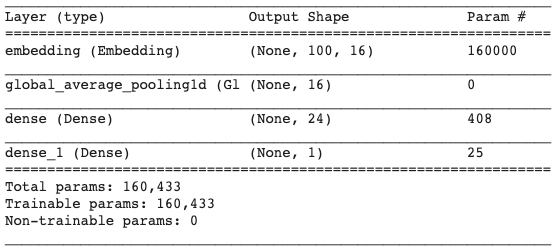
\includegraphics[width=250px]{img/AI/s.png}
    \caption{Summary del modelo AI}
    \label{fig:AI}
\end{figure} 

\begin{lstlisting}[style= mystyle, language=Python]
num_epochs = 30
history = model.fit(training_padded, training_labels, epochs=num_epochs, validation_data=(testing_padded, testing_labels), verbose=2)
\end{lstlisting}

Ahora realizaremos el entrenamiento de nuestra red neuronal. Para ello realizaremos 30 Epochs\footnote{Un Epoch es un término utilizado en Machine Learning que nos indica el número de pasadas del algoritmo al conjunto de entrenamiento.} a nuestro modelo AI. 


\begin{lstlisting}[style= mystyle, language=Python]
import matplotlib.pyplot as plt


def plot_graphs(history, string):
  plt.plot(history.history[string])
  plt.plot(history.history['val_'+string])
  plt.xlabel("Epochs")
  plt.ylabel(string)
  plt.legend([string, 'val_'+string])
  plt.show()
  
plot_graphs(history, "accuracy")
plot_graphs(history, "loss")
\end{lstlisting}

Ahora podremos visualizar el resultado de nuestro entrenamiento en la siguiente figura \ref{fig:AI} .
\begin{figure}[h!]
    \centering
    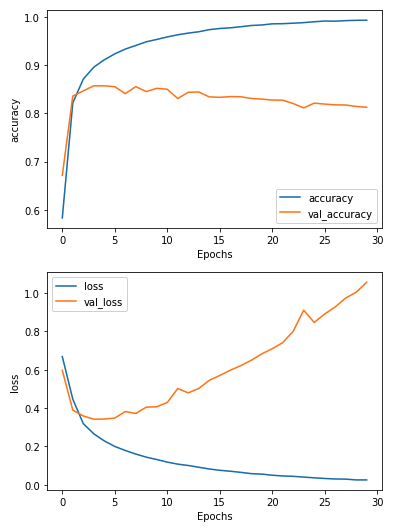
\includegraphics[width=250px]{img/AI/g.png}
    \caption{Resultado del entrenamiento de nuestra red neuronal}
    \label{fig:AI}
\end{figure} 

\begin{lstlisting}[style= mystyle, language=Python]
sentence = ["granny starting to fear spiders in the garden might be real", "game of thrones season finale showing this sunday night"]
sequences = tokenizer.texts_to_sequences(sentence)
padded = pad_sequences(sequences, maxlen=max_length, padding=padding_type, truncating=trunc_type)
print(model.predict(padded))
\end{lstlisting}

Finalmente, se podrá probar a continuación. Al correr model.predict(padded) obtenemos el siguiente vector: 
\begin{lstlisting}
[[9.0396011e-01]
 [8.0303380e-07]
 [4.1685485e-06]]\end{lstlisting}
 
 Esto quiere decir que existe una gran probabilidad de que la primera oración contenga sarcasmo, y una poca probabilidad que la segunda y tercera lo contenga.
 
 
\subsection{Futuras implementaciones y cambios para utilizar AI en la detección de ambigüedad}

La implementación mostrada en la última sección nos muestra el gran potencial de esta tecnología para resolver casos. Para poder aplicarlo con gramáticas, en la detección de ambigüedades, es necesario utilizar un modelo más complejo. Esto se debe a que ya no utilizaríamos como 'lable' a un número binario (0 y 1), por el contrario, tendríamos que utilizar otra estrategia. El arte de construir un modelo, está en definir de manera precisa el 'Embedding', con el objetivo de que los vectores generados cuenten con la presión deseada. Este arte, aplicado en el lenguaje natural, normalmente es propio de las grandes empresas; sin embargo en nuestra experimentación, nos empapamos con la tecnología detrás y la forma en la que esto funciona.
